%% template name: University of Agder - IKT Template %%

%% PREAMBEL %%
% Preamble
\documentclass[a4paper, 11pt]{article}

\title{}
\author{}

%% Pakker %%
% Språk
\usepackage[english]{babel}  % Norsk språk
\usepackage{csquotes}               % Anbefalt for babel
\usepackage{lipsum}                 % Pakke for fylltekst

% Bibliografi
\usepackage[backend=biber, style=ieee]{biblatex}
\addbibresource{bibliography.bib}
\usepackage[hidelinks]{hyperref}                % Lager lenker i TOC og bibliografi
\usepackage[nottoc]{tocbibind}
\setlength{\emergencystretch}{2em}

% Generelt
\usepackage[margin=25mm]{geometry}  % Pakke som kan endre layoutet til dokumentet
\usepackage{graphicx}               % Pakke som kan legge bilder i dokumentet
\usepackage{pdfpages}               % Pakke som kan legge pdf-filer i dokumentet
\usepackage{afterpage}
\newcommand\myemptypage{            % Lager en kommando som lager en ny side uten sidetall
    \null
    \thispagestyle{empty}
    \addtocounter{page}{-1}
    \newpage
}

\setlength{\parindent}{0em} % setter avsnittinnrykk til 0em
\setlength{\parskip}{1em} % setter avstanden mellom avsnitt til (NB! gjør ingenting da den blir overskrevet i innholdsfortegnelsen)

% Kodeblokker og plotting
\usepackage{pgfplots}                   % Pakke for linjediagrammer
\pgfplotsset{width=7cm, compat=newest}
\usetikzlibrary{patterns}
\usepackage{bchart}
\renewcommand{\bcfontstyle}{}
\usepackage{pgf-pie}                    
\usepackage{float}                      % Pakke for bedre posisjonering av figurer
\usepackage{setspace}
\usepackage{tabularx}
\usepackage{xcolor}
\usepackage{array} % added by fazal
\definecolor{codegreen}{rgb}{0,0.6,0}
\definecolor{codegray}{rgb}{0.5,0.5,0.5}
\definecolor{codepurple}{rgb}{0.68,0,0.12}
\definecolor{backcolour}{rgb}{0.96,0.96,0.96}

% Pakker for kodeblokker
\usepackage{listings}
\addto\captionsnorsk{\renewcommand{\lstlistlistingname}{Koder}}
\addto\captionsnorsk{\renewcommand{\lstlistingname}{Kode}}
\lstdefinestyle{mystyle}{
    backgroundcolor=\color{backcolour},
    commentstyle=\color{codegray},
    keywordstyle=\color{codepurple},
    numberstyle=\tiny\color{codegray},
    stringstyle=\color{codegreen},
    basicstyle=\ttfamily\footnotesize,
    breakatwhitespace=false,
    breaklines=true,
    captionpos=b,
    keepspaces=true,
    numbers=left,
    numbersep=5pt,
    showspaces=false,
    showstringspaces=false,
    showtabs=false,
    tabsize=2
}

\lstset{style=mystyle}

\author{Fazal Mahmud Niloy}

%% DOKUMENT START %%
\begin{document}

\pagenumbering{roman} % Sidenummerering for forord og TOC

%% FORSIDE %%
\begin{titlepage}
    \vbox{ }

    \vbox{ }

    \begin{center}
        % Øverste del av siden
        
\includegraphics[width=0.6\textwidth]{img/Uc-logo.png}\\[4cm]
        \textsc{\Large 11522 - ITS Capstone Project}\\[0.7cm]

        % \vbox{ }
        % Tittel
        \noindent\makebox[\linewidth]{\rule{.7\paperwidth}{.6pt}}\\[0.7cm]
        { \huge \bfseries An Analysis of Maternal and Neonatal Health Outcomes in Australia \& ACT: A Report on Australian \& ACT Mothers and Babies}\\[0.25cm]
        \noindent\makebox[\linewidth]{\rule{.7\paperwidth}{.6pt}}\\[0.7cm]
        \large{Semester 1, 2023}\\[1.2cm]
        \vfill
        % Forfatter
        \large
        % \emph{Skrevet av:}\\[1mm]
        Fazal Mahmud Niloy, Kanishka Goyal, Manisha Subba, Neha Pandey

        % Nederste del av siden
        {\large \today}
    \end{center}
\end{titlepage}

%% Declaration %%
% 

\large{\bf{Mandatory Group Declaration}}

{\small \hbadness=10000
Each student is solely responsible for familiarizing themselves with the legal aids, guidelines for their use, and rules regarding source usage. The declaration aims to raise awareness among students of their responsibilities and the consequences of cheating. Lack of declaration does not exempt students from their responsibilities.

\begin{center}
\begin{tabular}{ |p{0.2cm}|p{13.5cm}|p{1cm}|}
\hline

1.& We hereby declare that our submission is our own work and that we have not used other sources or received any help other than what is mentioned in the submission. & Yes / No \\
\hline
2. & \textbf{We further declare that this submission:}
\begin{itemize}
\item Has not been used for any other examination at another department/university/college domestically or abroad.
\item Does not reference others' work without it being indicated.
\item Does not reference our own previous work without it being indicated.
\item Has all references included in the bibliography.
\item Is not a copy, duplicate, or transcription of others' work or submission.
\end{itemize}& Yes / No \\
\hline
3. & We are aware that violations of the above are considered to be cheating and can result in cancellation of the examination and exclusion from universities and colleges in Norway, according to the Universities and Colleges Act, sections 4-7 and 4-8 and the Examination Regulation, sections 31.
 & Yes / No \\
\hline
4. & We are aware that all submitted assignments may be subjected to plagiarism checks.
& Yes / No \\
\hline
5. & We are aware that the University of Agder will handle all cases where there is suspicion of cheating according to the university's guidelines for handling cheating cases.
& Yes / No \\
\hline
6. & We have familiarized ourselves with the rules and guidelines for using sources and references on the library's website.
& Yes / No \\
\hline
7. & We have in the majority agreed that the effort within the group is notably different and therefore wish to be evaluated individually.
Ordinarily, all participants in the project are evaluated collectively.
& Yes / No \\
\hline
\end{tabular}
\end{center}
}

\large{\textbf{Publishing Agreement}}

{\small \hbadness=10000 Authorization for Electronic Publication of Work
The author(s) hold the copyright to the work. This means, among other things, the exclusive right to make the work available to the public (Copyright Act. §2).

Theses that are exempt from public access or confidential will not be published.\\
\begin{center}
\begin{tabular}{ |p{10cm}|p{3cm}|}
\hline
We hereby grant the University of Agder a royalty-free right to make the work available for electronic publication: & Yes / No \\
\hline
Is the work confidential? & Yes / No \\
\hline
Is the work exempt from public access? & Yes / No \\
\hline
\end{tabular}
\end{center}
}


%% INNHOLDSFORTEGNELSE %%
\setlength{\parskip}{.5em} % Setter linjeavstander i TOC litt mindre
\cleardoublepage
\tableofcontents
\setlength{\parskip}{1em} % Går tilbake til standard avstand
\newpage

%% SAMMENDRAG & FORORD %%

\pagenumbering{arabic} % Sidenummerering for resten av dokumentet

%% SEKSJONER %%
\section{Abstract}
This paper presents an analysis of maternal and neonatal health outcomes in Australia, with a focus on the health status of Australian mothers and babies. The study utilized data from various sources including government statistics, research studies, and national surveys to provide a comprehensive overview of the current state of maternal and neonatal health in Australia.

The report highlights that despite improvements in maternal and neonatal health outcomes in recent years, Australia still faces significant challenges in reducing maternal and neonatal mortality rates, particularly among disadvantaged groups. The analysis also reveals significant disparities in health outcomes among different demographic groups, including Aboriginal and Torres Strait Islander communities and women living in remote and rural areas.

The paper examines various factors that contribute to maternal and neonatal health outcomes, including access to healthcare services, social determinants of health, and lifestyle factors. It also discusses the implications of these findings for healthcare policy and practice in Australia.

Overall, this paper underscores the importance of continued efforts to improve maternal and neonatal health outcomes in Australia, particularly for vulnerable populations. The analysis provides a valuable resource for policymakers, healthcare providers, and researchers seeking to address the complex challenges of maternal and neonatal health in Australia.
\section{Introduction}
Maternal and neonatal health outcomes are important indicators of a society's overall health and well-being. In recent years, there has been a growing interest in understanding the health status of mothers and babies in Australia. This paper provides a comprehensive analysis of maternal and neonatal health outcomes in Australia, focusing on the health status of Australian mothers and babies.

The report draws on a range of sources, including the Australian Institute of Health and Welfare(AIHW), the Australian Bureau of Statistics (ABS), and the National Perinatal Data Collection to provide a comprehensive overview of the current state of maternal and neonatal health in Australia. The analysis aims to identify key challenges and areas of progress in maternal and neonatal health, as well as the factors that contribute to these outcomes.

Despite significant improvements in maternal and neonatal health outcomes in recent years, there are still significant disparities in health outcomes among different demographic groups in Australia. These disparities are particularly pronounced among disadvantaged groups, including Aboriginal and Torres Strait Islander communities and women living in remote and rural areas. The analysis also reveals that lifestyle factors, access to healthcare services, and social determinants of health are important contributors to maternal and neonatal health outcomes in Australia.

The findings of this paper have important implications for healthcare policy and practice in Australia. By identifying key challenges and areas of progress in maternal and neonatal health, this report provides a valuable resource for policymakers, healthcare providers, and researchers seeking to improve maternal and neonatal health outcomes in Australia. 
\section{Scopes}
\begin{enumerate}
    \item  Examine various maternal characteristics and medical histories associated with mother and babies’ health, such as maternal age, ethnicity, socioeconomic status, parity, pre-existing medical conditions, and pregnancy complications.
    \item  Inspect the trends of maternal and perinatal mortality, such as the period of occurrence prenatal, intrapartum, or postpartum.
    \item Explore the trends across different decades and between different states of Australia.
    \item Analyze long-term trends that could provide insight into the effectiveness of existing policies and programs, and identify areas where further improvements are needed.
    \item Build a dynamic dashboard for visualization and modeling purposes.
\end{enumerate}


\section{Project Requirements}
Requirements for this project included:
\subsection{Data Sources}
\begin{itemize}
%% will change this section
  \item Since this project aims to work alongside AIHW the team has considered AIHW as their primary data source. Although, the data available on the AIHW website are summary or aggregated data and it does not include individual records. Their 3 primary data sources which are National Perinatal Data Collection, National Perinatal Mortality Data Collection \& National Maternal Mortality Data Collection’s data can be accessed by making a request with table specifications to the data provider.
  \item Our team wants to use the Australian Bureau of Statistics data on birth as a secondary dataset. These datasets have records from 1991-2021 of birth data. It includes the data describing the parent’s birthplace, age, ethnicity if they are aboriginal, birthrate of the area, etc which can play vital roles in this project’s analysis.
\end{itemize}

\subsection{Budget}
The allocated budget of AUD300 was not used since the data was not accessible and a request for data was not made as our sponsor indicated that by the time our request would be fulfilled and get the data in our hands, the project will also reach its deadline.

\section{Methodology}
In order to perform analysis on the available data we used \verb|R studio|. After loading the datasets to a suitable dataframe format rigorous cleanup was performed since the data was not ideal for our scope of analysis. After we got the cleaned data for each analysis and/or step statistical analysis and shaping were performed so that it becomes easy to interface the data to its related tool such as \verb|plotly|, \verb|ggplot|. After feeding the shaped data to these tools we get human-readable visualizations that can be easily interpreted and inferred. Sections below are the observations we have found from our analysis.
\section{Used Resources}
\subsection{Hardware Resources}
 No external hardware was required. The use of each individual's machine had been decided for data analysis, visualization, forecasting, etc. In the case of dealing with robust data, the remote computers from the university laboratory had been considered, which had capable Nvidia GPUs for the tasks displayed in the report.
\subsection{Software Resources}
\begin{itemize}
    \item Rstudio
    \item Pycharm
    \item Python 3.8
    \item Microsoft Excel
    \item Git for version controlling and contribution management
    \item Discord for internal team communication
\end{itemize}

\section{Project Resources}
Requirements for this project include
\subsection{Data Sources}
\begin{itemize}
    \item Since this project aims to work alongside AIHW the team has considered AIHW as their primary data source. Although, the data available on the AIHW website are summary or aggregated data and it does not include individual records. Their 3 primary data sources which are National Perinatal Data Collection, National Perinatal Mortality Data Collection \& National Maternal Mortality Data Collection’s data can be accessed by making a request with table specifications to the data provider.
    \item Our team wants to use the Australian Bureau of Statistics data on birth as a secondary dataset. These datasets have records from 1991-2021 of birth data. It includes the data describing parent’s birthplace, age, ethnicity if they are aboriginal, the birthrate of the area, etc which can play vital role in this project’s analysis.
\end{itemize}
\subsection{Budget}
The 3 different data sources do not mention any price per record but from the team’s understanding, it is assumed that the allocated AUD300 should cover the data requested from the sources. Since no new hardware is required for the completion of this project, no budget is being considered for purchasing or gaining access to new hardware.

\section{Findings}
\subsection{Age of Mothers}
Our first aim was to have an overall understanding of the mothers' age group and their proportions. After performing some statistical analysis we get two figures that show the trends of mothers of different age groups in different states as well as overall Australia. It can be observed that in most Australian states women who are aged less than 20 make the most proportion of mothers. After them, mothers who are 40 or more make up the 2nd largest age group (figure \ref{fig:age0.1}). Mothers from the age group of 20-24 make up the second biggest sample if we look at individual data from different states (figure \ref{fig:age0.2}). However, in (Figure: \ref{fig:age1}) ACT we see a different trend in data. We can see that the age group of 15-19 and over 40 are the last 2 age groups while most mothers are from the age group of 30-34. 

\begin{figure}
  \centering
  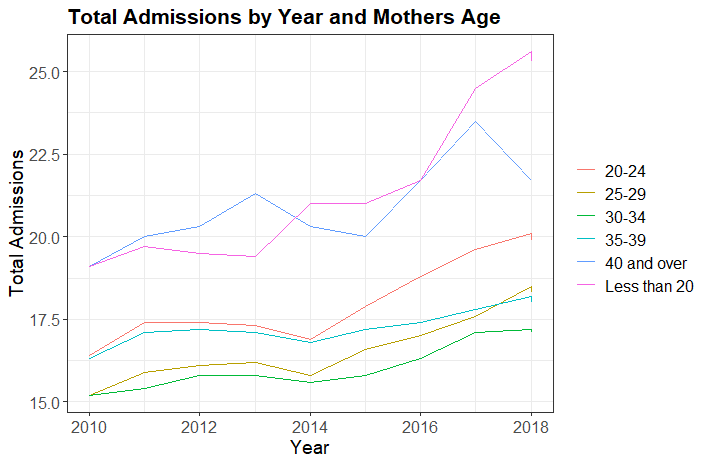
\includegraphics[width=1\textwidth]{subsections/age_mothers/mothers_age.png}
  \caption{Proportion of mothers by different age groups in Australia.}
  \label{fig:age0.1}
\end{figure}

\begin{figure}
  \centering
  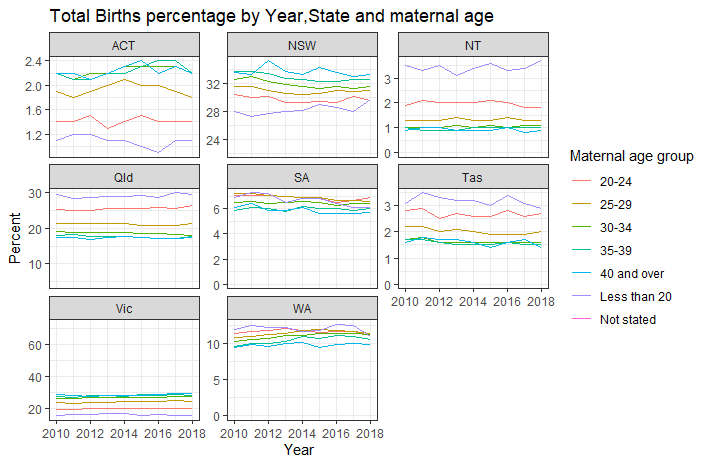
\includegraphics[width=1\textwidth]{subsections/age_mothers/birth_age_state.png}
  \caption{Proportion of mothers by different age groups in different states.}
  \label{fig:age0.2}
\end{figure}

\begin{figure}
  \centering
  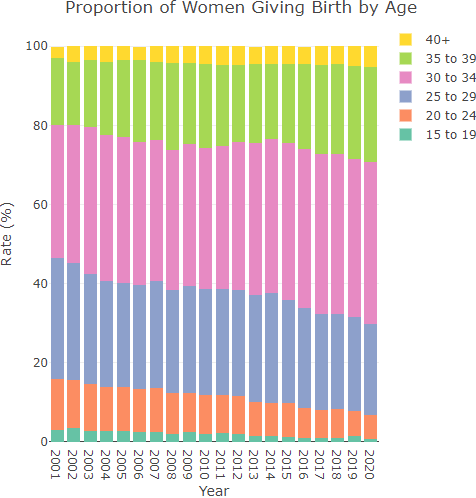
\includegraphics[width=0.50\textwidth]{subsections/age_mothers/age_group.png}
  \caption{Proportion of woman giving birth by age in ACT.}
  \label{fig:age1}
\end{figure}
\subsubsection{Analysis: First Time Mothers of ACT}

\begin{figure}
  \centering
  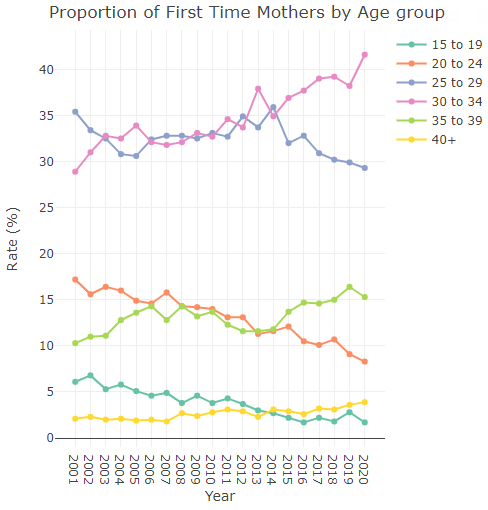
\includegraphics[width=0.5\textwidth]{subsections/age_mothers/first_time_age_group.png}
  \caption{Trends of first-time mother by age group.}
  \label{fig:age2}
\end{figure}

\begin{figure}
  \centering
  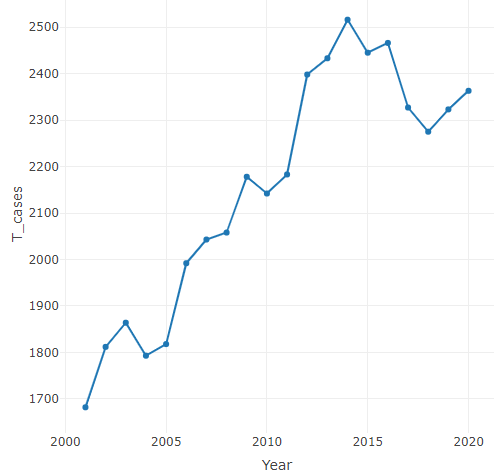
\includegraphics[width=0.45\textwidth]{subsections/age_mothers/first_time.png}
  \caption{Number of first-time mothers in each year.}
  \label{fig:firstTime}
\end{figure}
For a deeper understanding of what we have found in \verb|section 5.2| we were interested to see how many women became mothers for the first time. To achieve that we have generated Figure: \ref{fig:age2} where we can see that although mothers who are aged 40+ tend to have babies less the trend has been changing from the last decade and they have more birthrate than the age group of 15-19 years old. The low birthrate of 15-19 is understandably low as the legal age of consent is 16 except for Tasmania and South Australia which is 17 \cite{consentWebsite}.

Intuitively, this analysis leads us to ask how many women were becoming mothers for the first time each year so that we can observe a trend in women having babies. After generating figure: \ref{fig:firstTime} we can see that number of women becoming first-time mothers has increased over the years.

\subsection{Method of Birth}
Methods of birth can be classified into 4 categories. They are:
\begin{enumerate}
    \item Cesarean section
    \item Vaginal (forceps)
    \item Vaginal (non-instrumental)
    \item Vaginal (vacuum)
\end{enumerate}
If we look at the overall data in Figure \ref{fig:method_au} of Australia we can see that as time passed all of these births of different methods are increasing but the number of vaginal birth has increased more over time in comparison with other methods.
\begin{figure}
  \centering
  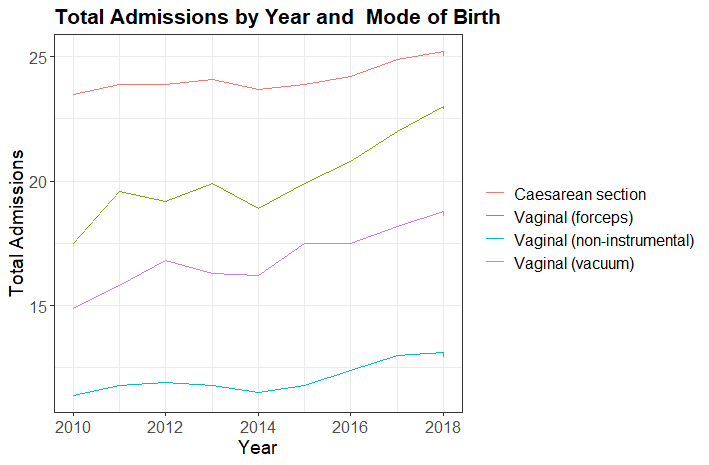
\includegraphics[width=0.75\textwidth]{subsections/method_of_birth/method_of_birth_au.png}
  \caption{Method of births in Australia over the years.}
  \label{fig:method_au}
\end{figure}
\subsubsection{Analysis: Onset Labour in ACT}
The onset of labor refers to the beginning of the active phase of labor, which is the process by which the uterus contracts and the cervix dilates to allow for the delivery of a baby. This is typically considered to occur when regular and frequent contractions begin, and the cervix starts to dilate and efface (thin out)\cite{birthColum}.

The onset of labor can vary from woman to woman and pregnancy to pregnancy. Some women may experience a gradual onset of contractions over several days, while others may have a sudden onset of strong and frequent contractions. The onset of labor can be influenced by a variety of factors, including hormones, fetal position, and maternal health. 

\begin{figure}
  \centering
  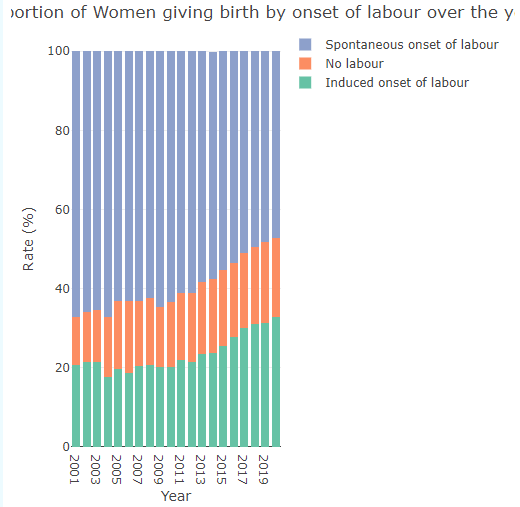
\includegraphics[width=0.45\textwidth]{subsections/method_of_birth/onset_method.png}
  \caption{Proportion of woman of ACT giving onset birth.}
  \label{fig:onset}
\end{figure}

\begin{figure}
  \centering
  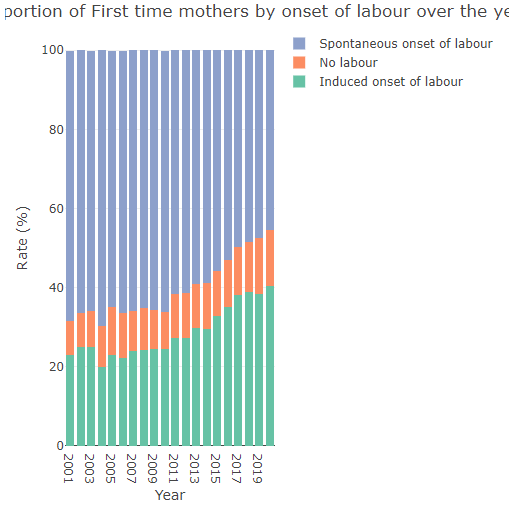
\includegraphics[width=0.45\textwidth]{subsections/method_of_birth/onset_method_first_time.png}
  \caption{Proportion of first-time mothers of ACT giving onset birth.}
  \label{fig:onsetFirsttime}
\end{figure}

To have a look at the data of mothers giving onset birth over the years we looked at the proportion and were curious to find out how the pattern changed. According to our observation, which is shown in Figures \ref{fig:onset} and \ref{fig:onsetFirsttime}, it is observed that spontaneous onset labour has decreased in last two decades while on the other hand, induced labour has increased over the years. We can see similar trends in the first-time mothers' data but the proportion of having no labour decreases significantly.
\subsubsection{Vaginal Births in ACT}
Vaginal birth, also known as normal vaginal delivery, is the natural way for a baby to be born through the birth canal. It offers several significant benefits for both the mother and the baby, including:

\begin{itemize}
  \item Quicker recovery: Vaginal birth typically has a shorter recovery time than a cesarean section, which is a surgical delivery. Mothers who have vaginal births can usually go home from the hospital sooner, and they often experience less pain and discomfort during the recovery period.
  \item Fewer complications: Vaginal birth is associated with fewer complications for both the mother and the baby compared to cesarean section. For example, the risk of infection, blood loss, and injury to internal organs is lower with vaginal birth.
  \item Better for breastfeeding: Babies who are born vaginally are more likely to have an easier time breastfeeding. This is because the pressure of passing through the birth canal helps to expel fluid from the baby's lungs and stimulates the release of hormones that help with breastfeeding.
  \item Improved gut health: Babies born vaginally also tend to have a healthier gut microbiome compared to those born via cesarean section. The bacteria that the baby is exposed to during vaginal birth can help to colonize the gut and support a healthy immune system.
  \item Psychological benefits: Some mothers report feeling a greater sense of empowerment and satisfaction after having a vaginal birth. This may be due to the sense of achievement and control that comes with delivering a baby without medical intervention.
\end{itemize}

Overall, vaginal birth is a safe and natural option for most women, and it offers several significant benefits for both the mother and the baby. However, it's important for each woman to discuss her individual medical history and pregnancy with her healthcare provider to determine the best course of action for her delivery.

We can see in figure \ref{fig:vaginal_act} Cesarean section method is more prominent among mothers who are over 40. Oppositely we can observe that younger women mostly have vaginal births. As the age increases the number of vaginal birth decreases and cesarean section increases.

\begin{figure}
  \centering
  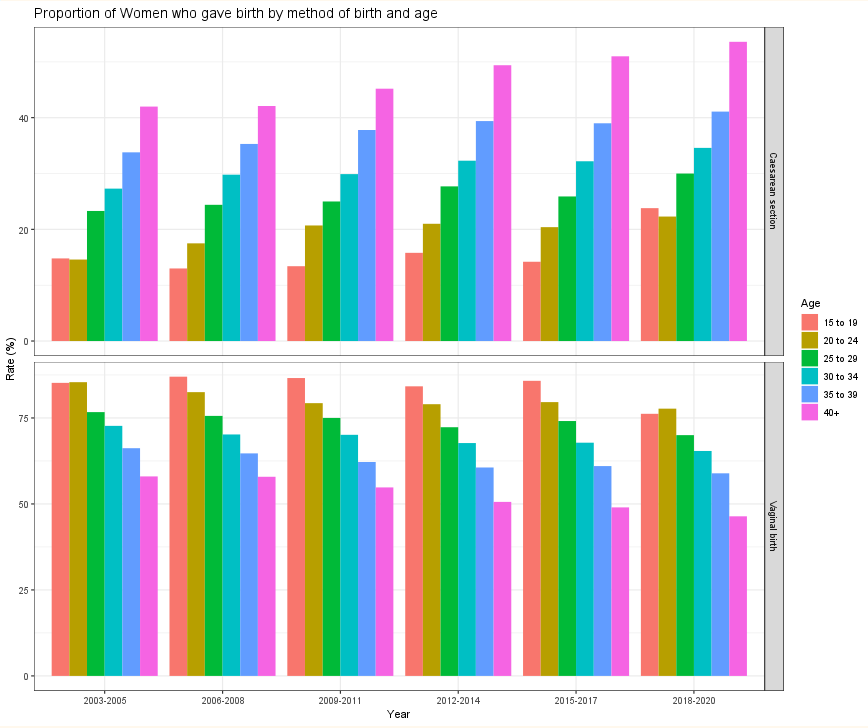
\includegraphics[width=1\textwidth]{subsections/method_of_birth/vagina_proportion.png}
  \caption{Different methods of birth in different mothers of different age groups (ACT).}
  \label{fig:vaginal_act}
\end{figure}
\subsection{Socioeconomic Status}
Socioeconomic status can play a crucial role in terms of the ability to afford healthcare, access to doctors \& medication, healthy food etc. Interestingly, in figure \ref{fig:socioecoau} we can see that through the years the most disadvantaged mothers had babies. To have a deeper insight we looked into state-based data. We can see (figure\ref{fig:socioecostates}) different trends in different states. We can observe that in some states such as ACT, NSW \& NT more advantaged the mothers are more interested they are in having babies. Interestingly, we can see the opposite trend in QLD, SA \& Tasmania where often the least advantaged mothers tend to have more babies.

\begin{figure}
  \centering
  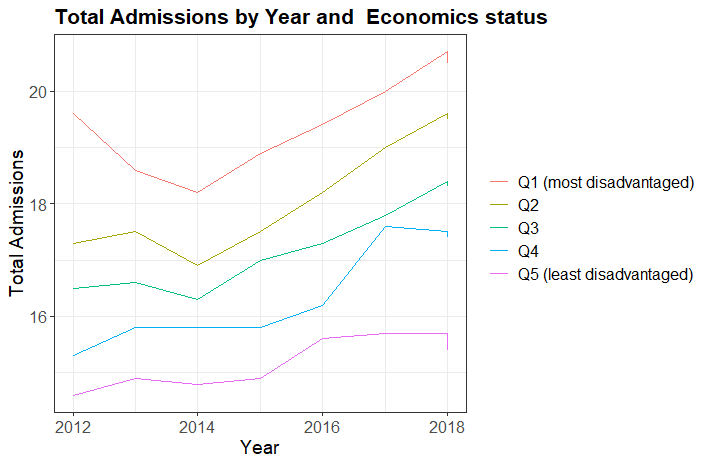
\includegraphics[width=1\textwidth]{subsections/socioeco/economic_status_au.png}
  \caption{Socioeconomic status of mothers in Australia.}
  \label{fig:socioecoau}
\end{figure}

\begin{figure}
  \centering
  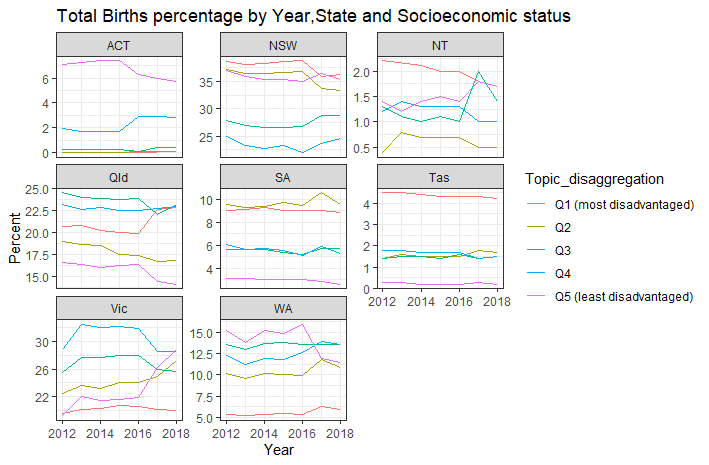
\includegraphics[width=1\textwidth]{subsections/socioeco/socio_economic.png}
  \caption{Socioeconomic status of mothers in different states.}
  \label{fig:socioecostates}
\end{figure}
\subsection{Baby \& Mother's Health}
The baby's and mother's health is an important factor during and after childbirth. Successful childbirth often depends on some key factors of the baby's health such as gestational age, the weight of the baby when it was born, etc. To analyze this we looked into the Australian dataset (figure \ref{fig:bmi_au}) and we can observe that the majority of the babies were underweight at the time they were born. It can often happen as sometimes doctors suggest mothers be conservative about eating during the last stage of pregnancy as the labour can become very difficult if the baby is overweight \emph{[citation needed]}.
\begin{figure}
  \centering
  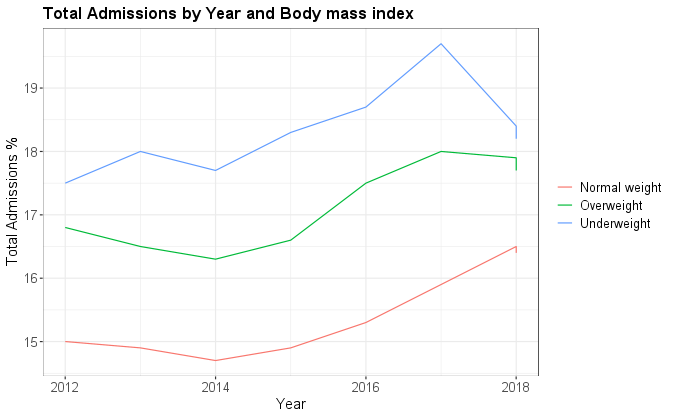
\includegraphics[width=0.75\textwidth]{subsections/baby_health/bmi.png}
  \caption{BMI of babies in Australia over the years.}
  \label{fig:bmi_au}
\end{figure}
Below are the findings we get after analysing data that focuses on ACT data only.

\subsubsection{Gestational Age of Babies in ACT}
Gestational age refers to the amount of time a fetus has spent in the womb, starting from the first day of the mother's last menstrual period. It is typically measured in weeks and is used to track fetal development and monitor the progress of pregnancy.

Babies born between 37 and 40 weeks are considered full-term and are generally at a lower risk for complications than those born earlier. These babies have had enough time to develop and mature in the womb, which can help ensure that they are able to breathe, eat, and maintain their body temperature after birth.

Babies born before 37 weeks are considered premature and may require special care and monitoring in a neonatal intensive care unit (NICU). Premature babies are at a higher risk for a range of complications, including respiratory distress syndrome, jaundice, and infections.

On the other hand, babies born after 40 weeks are considered post-term and may also be at a higher risk for complications, such as macrosomia (large birth weight), meconium aspiration syndrome, and fetal distress. In these cases, medical professionals may recommend inducing labor to ensure the health and safety of both the mother and the baby.

\begin{figure}
  \centering
  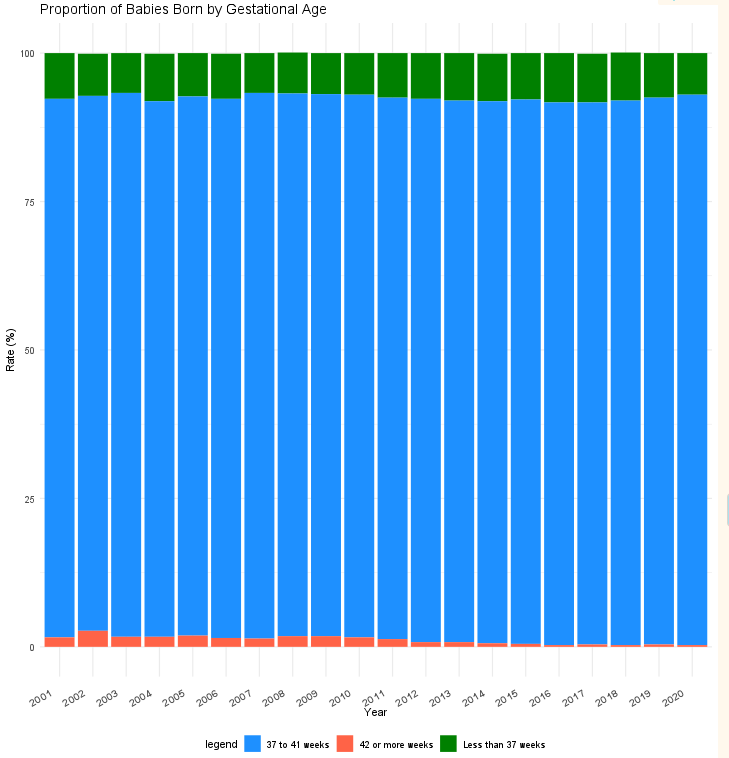
\includegraphics[width=0.8\textwidth]{subsections/baby_health/gestational_age_act.png}
  \caption{Gestational age of babies in ACT.}
  \label{fig:gest_act}
\end{figure}

In \textbf{Figure \ref{fig:gest_act}} we can see that the gestational age of babies has been really good which is over 90\%.
\subsubsection{Underweight Newborn of Babies in ACT}
Ideally, a baby is considered underweight if its weight is less than 2500 grams. In order to determine how ACT is doing in this regard we generated a visualization that shows the percentage of babies who are underweight grouped by their gestational age \textbf{(figure \ref{fig:weight_gest})}. We can see that most of the underweight babies born are from the ideal gestational period. This may seem misleading but can be explained if we look at \textbf{figure \ref{fig:gest_act}} we can see that 90\% of the babies are born in that group which explains the disproportionate amount of babies in ACT being born underweight.

\begin{figure}
  \centering
  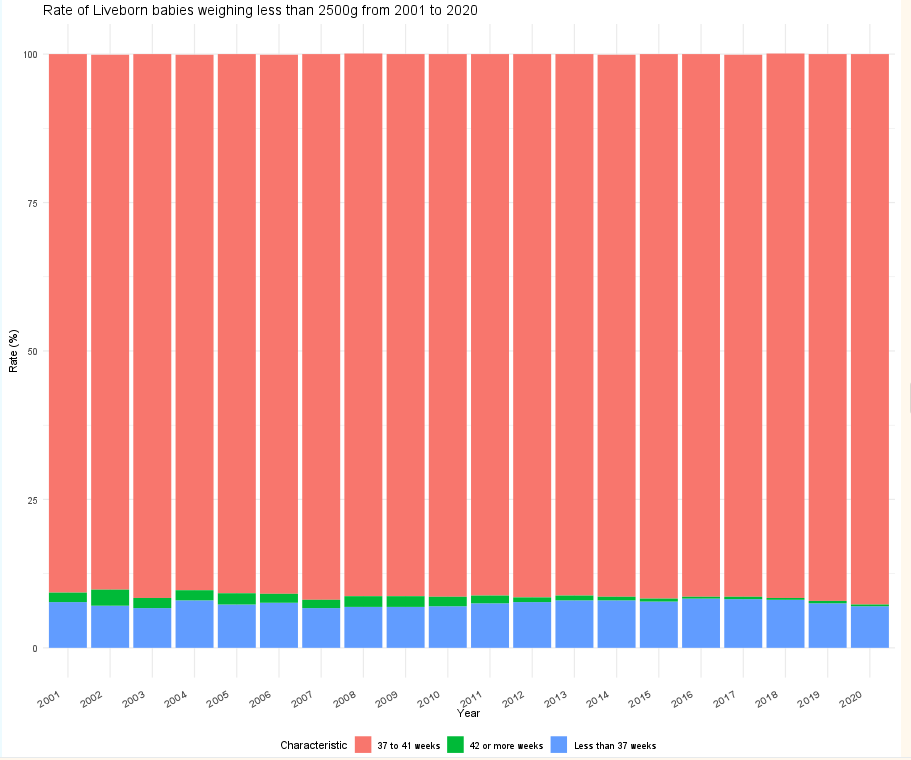
\includegraphics[width=0.8\textwidth]{subsections/baby_health/live_born_weigh_proportion_act.png}
  \caption{Liveborn baby weight proportion in ACT.}
  \label{fig:weight_gest}
\end{figure}

In \textbf{Figure \ref{fig:weight_act}} we can also see that even though the rate of underweight babies is around 5\% through the years it is showing an upward trend.

\begin{figure}
  \centering
  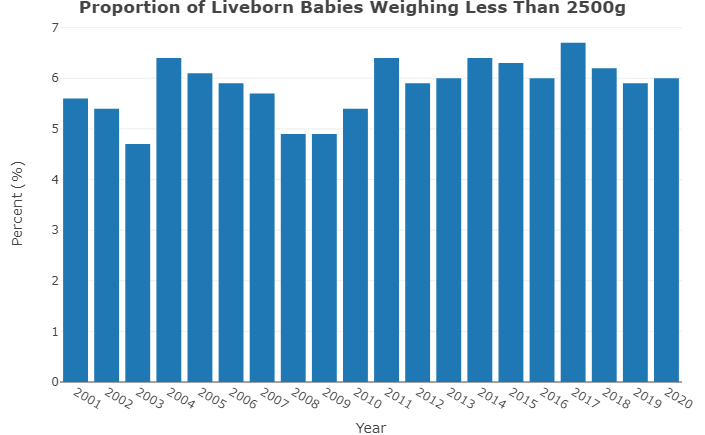
\includegraphics[width=0.8\textwidth]{subsections/baby_health/liveborn_weight.png}
  \caption{Underweight babies weight}
  \label{fig:weight_act}
\end{figure}
\subsubsection{Mother's Gestational Diabetes}
Gestational diabetes is a type of diabetes that occurs during pregnancy. It affects about 2-10\% of pregnant women and usually develops in the second or third trimester of pregnancy. Gestational diabetes can increase the risk of complications during pregnancy and delivery, as well as the risk of developing type 2 diabetes later in life.

The exact cause of gestational diabetes is not fully understood, but it is thought to be related to hormonal changes that occur during pregnancy. During pregnancy, the placenta produces hormones that can interfere with the body's ability to use insulin effectively. Insulin is a hormone that regulates blood sugar levels, and when the body is unable to use insulin properly, blood sugar levels can become elevated, leading to gestational diabetes.

Women who are at increased risk of developing gestational diabetes include those who are overweight or obese, have a family history of diabetes, have previously had gestational diabetes, have polycystic ovary syndrome (PCOS), or are older than 25 years of age.

Treatment for gestational diabetes usually involves dietary changes, such as reducing the intake of simple sugars and increasing the intake of complex carbohydrates, as well as regular exercise. In some cases, insulin injections may also be needed to control blood sugar levels. It is important for women with gestational diabetes to monitor their blood sugar levels regularly and attend all prenatal appointments to ensure that both they and their babies are healthy.

In \textbf{figure \ref{fig:gest_diabetes}} we can see a sudden spike in gestational diabetes among mothers in ACT.

\begin{figure}
  \centering
  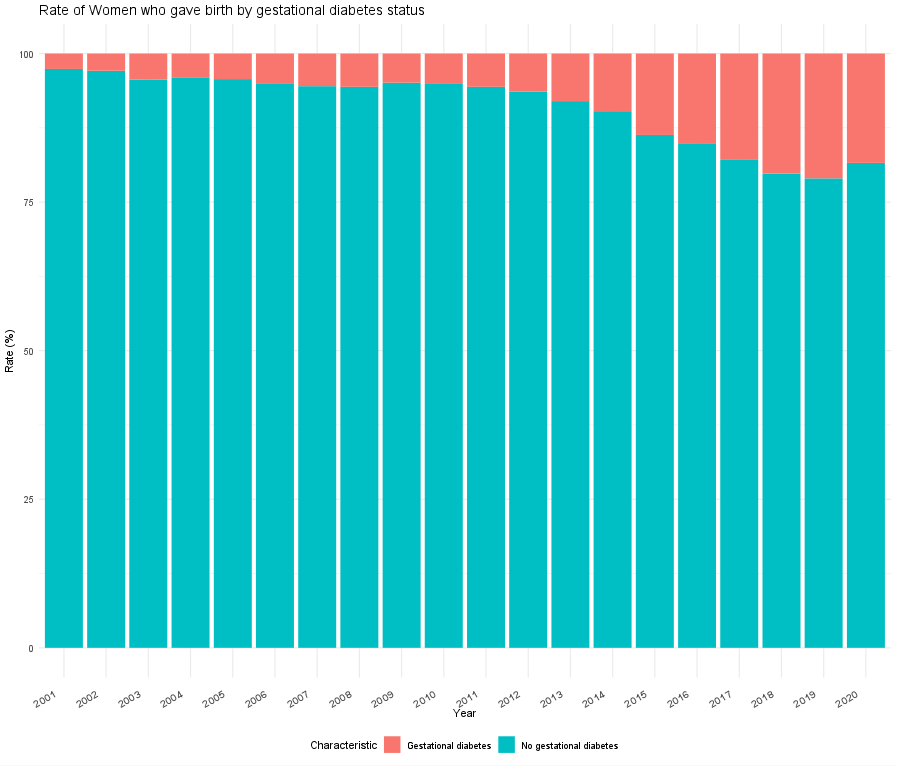
\includegraphics[width=0.90\textwidth]{subsections/baby_health/gestational_diabetes_rate.png}
  \caption{Gestational diabetes rate of mothers in ACT.}
  \label{fig:gest_diabetes}
\end{figure}
\subsection{Neonatal \& Perinatal Deaths and Stillbirths}
Neonatal refers to the first 28 days of life after birth. This is a critical period for the baby's development, and neonatal care is essential to ensure their survival and well-being.

Perinatal refers to the period of time surrounding the birth of a baby, typically starting at 22 weeks of gestation and ending seven days after birth. This period includes both the antepartum (before birth) and intrapartum (during birth) periods.

Stillbirth is the term used when a baby is born without signs of life after 20 weeks of gestation. This can happen before, during, or after delivery. Stillbirth is a devastating loss for parents and families and is often a traumatic experience.

In Australia, perinatal deaths are relatively rare, but they remain a significant public health issue.

If we look at the Australia-wide data \textbf{figure \ref{fig:neo-rate}}, \textbf{figure \ref{fig:peri-rate}} \& \textbf{figure \ref{fig:still-rate}} we can see that the neonatal, perinatal, and stillbirth rate are decreasing through the years

\begin{figure}
  \centering
  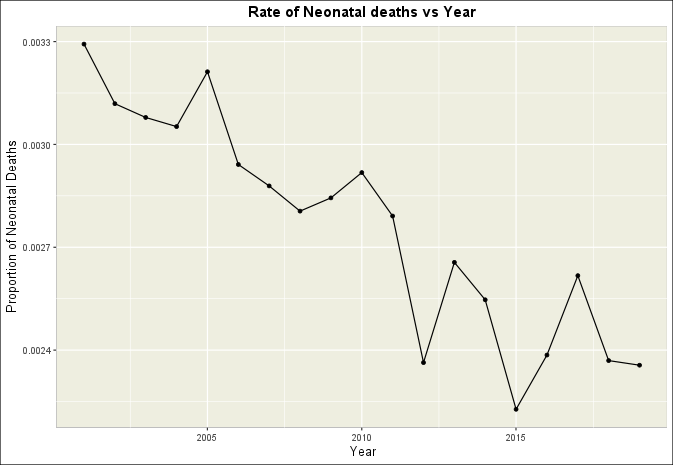
\includegraphics[width=.5\textwidth]{img/aus/kanishka/neonatal_deaths.png}
  \caption{neonatal death rate}
  \label{fig:neo-rate}
\end{figure}

\begin{figure}
  \centering
  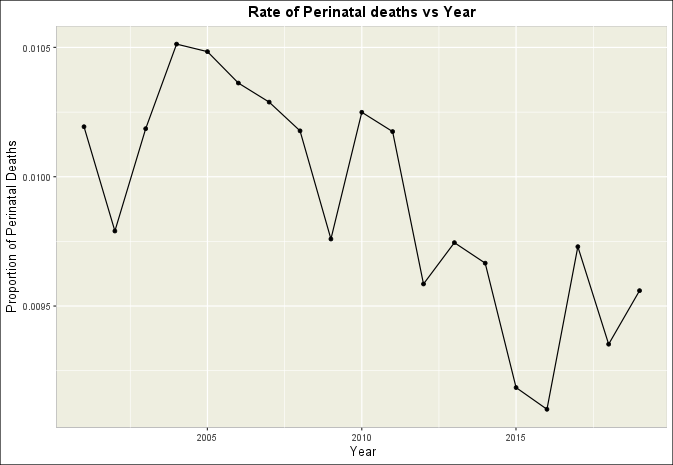
\includegraphics[width=.5\textwidth]{img/aus/kanishka/perinatal_deaths.png}
  \caption{neonatal death rate}
  \label{fig:peri-rate}
\end{figure}

\begin{figure}
  \centering
  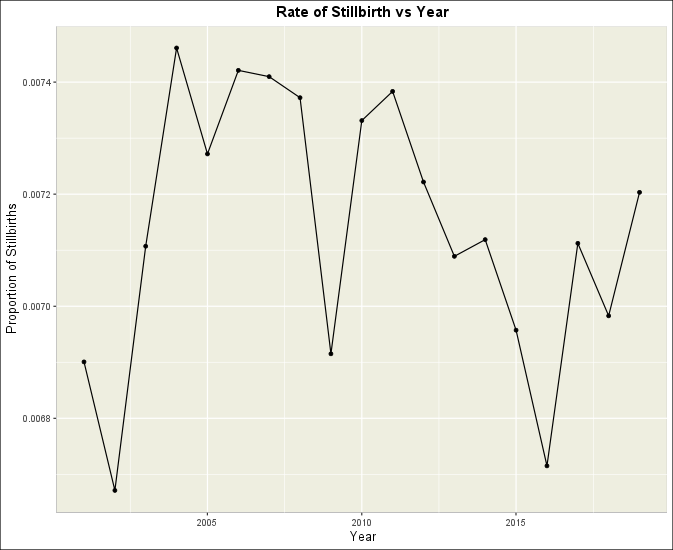
\includegraphics[width=.5\textwidth]{img/aus/kanishka/stillbirth_year.png}
  \caption{stillbirth rate}
  \label{fig:still-rate}
\end{figure}

\subsubsection{Perinatal Deaths vs Mothers' Age}
Perinatal deaths can also happen because of mothers' health factors such as age. To identify how age is contributing to perinatal death we have generated \textbf{Figure \ref{fig:peri_mother}} to try to understand the trend of the data. We can see that perinatal death is significantly high among mothers who are aged below 20. The second biggest group, in this case, is mothers who are aged 40 and over. The group that has consistently low perinatal death is mothers who are aged between 30-34.
\begin{figure}
  \centering
  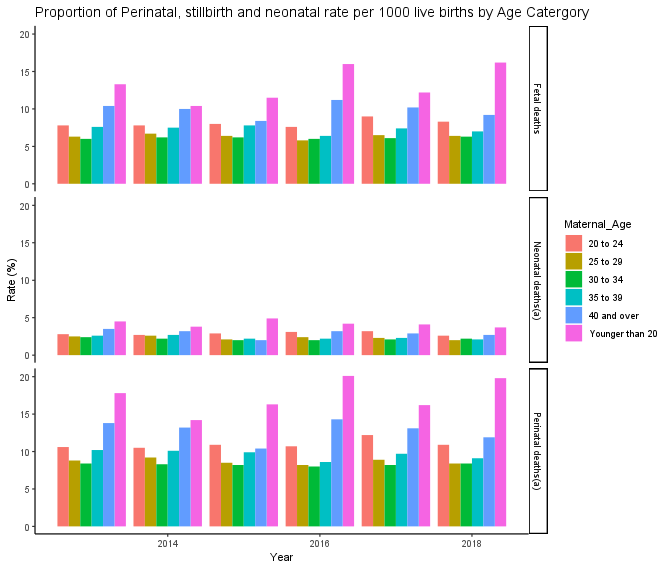
\includegraphics[width=.75\textwidth]{subsections/perinatal_deaths/by_mother_age_baby_death.png}
  \caption{Perinatal death vs Maternal age}
  \label{fig:peri_mother}
\end{figure}
\subsubsection{Child Deaths vs Socio-Economic Area \& Remoteness}
Successful childbirth often depends on parents' socio-economical status \& geographical location since those determine accessibility to better healthcare, medication better antinatal visiting practices.

In \textbf{Figure \ref{fig:peri_state}} we can see that in Queensland and New South Wales, the perinatal death has always been low but in Northern Territory, it has been high through the years. The graph also shows that neonatal deaths are significantly low in every state through the years compared to stillbirths.
\begin{figure}
  \centering
  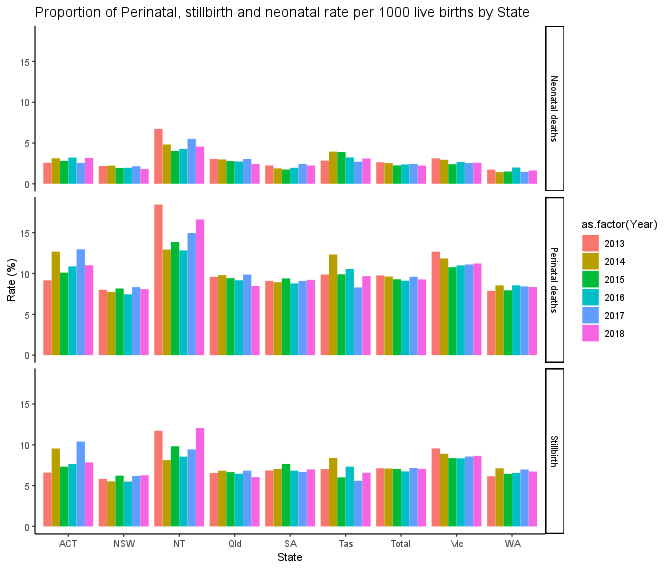
\includegraphics[width=.75\textwidth]{subsections/perinatal_deaths/by_state_birth_baby_death.png}
  \caption{Perinatal death rate per year}
  \label{fig:peri_state}
\end{figure}

To have a deeper understanding, we look into the mother's socio-economic area in \textbf{figure \ref{fig:mother_res}}. Q1 means the most disadvantaged area and Q5 means the least disadvantaged area. It can be clearly observed that the most disadvantaged area has a high mortality rate for all categories of deaths and the least disadvantaged area has the least mortality rate.

\begin{figure}
  \centering
  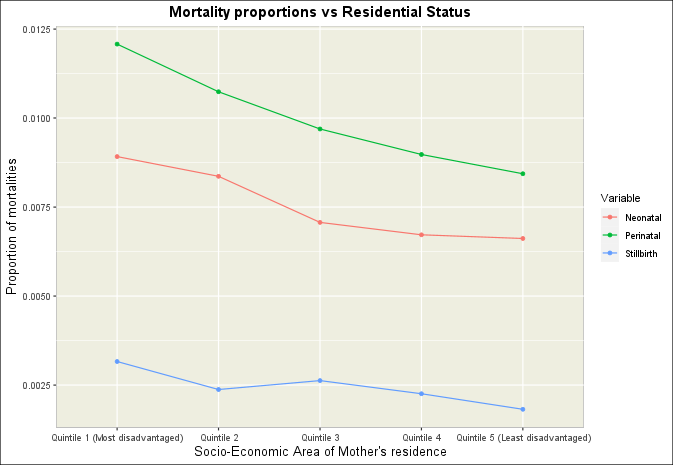
\includegraphics[width=.75\textwidth]{img/aus/kanishka/mortality_residentialStat.png}
  \caption{Socio-economic area of mother's residence}
  \label{fig:mother_res}
\end{figure}

Following that, we wanted to see how the mortality rate was in remote areas in comparison with major cities which are more developed (\textbf{figure \ref{fig:mother_res_remoteness}}). It can be seen that the "Very Remote" areas have the most mortality rate on the other hand major cities have the least death rate.

\begin{figure}
  \centering
  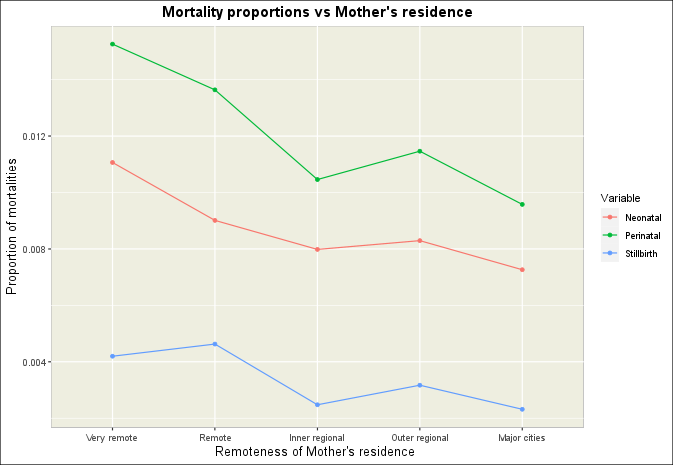
\includegraphics[width=.75\textwidth]{img/aus/kanishka/mortality_mothers_res.png}
  \caption{Remoteness of mother's residence}
  \label{fig:mother_res_remoteness}
\end{figure}
\subsection{Smoking Habits Among Mothers}
The mothers' smoking habit during pregnancy can have a range of negative effects on both the mother and the developing fetus. Some of the potential effects of smoking during pregnancy include:

\begin{enumerate}
    \item Increased risk of miscarriage: Smoking during pregnancy increases the risk of miscarriage, especially during the first trimester.
    \item Preterm delivery: Smoking during pregnancy can increase the risk of delivering the baby before 37 weeks of gestation, which can lead to a range of health problems for the baby.
    \item Low birth weight: Babies born to mothers who smoke during pregnancy are more likely to have a low birth weight, which can lead to a range of health problems, including developmental delays, infections, and breathing difficulties.
    \item Sudden infant death syndrome (SIDS): Babies born to mothers who smoke during pregnancy are at a higher risk of SIDS, which is the sudden and unexplained death of an otherwise healthy baby.
    \item Respiratory problems: Smoking during pregnancy can cause respiratory problems for the developing fetus, including asthma and other lung diseases.
    \item Behavioral problems: Children born to mothers who smoke during pregnancy may be more likely to experience behavioral problems, such as ADHD and conduct disorder.
\end{enumerate}

It's important for mothers to quit smoking during pregnancy to protect the health of their developing fetus and their own health as well. If you're a smoker and pregnant, you should talk to your doctor about strategies for quitting smoking and improving the health of your baby.

In overall Australia, we can see \textbf{(figure \ref{fig:smoking_au})} that mothers who smoked has increased in number.
\begin{figure}
  \centering
  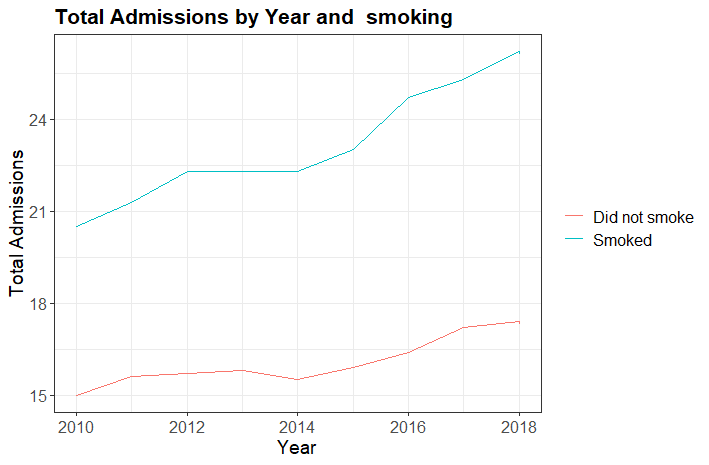
\includegraphics[width=.75\textwidth]{subsections/smoking/smoking_aus.png}
  \caption{Mother's smoking habit in ACT}
  \label{fig:smoking_au}
\end{figure}

Oppositely \textbf{figure \ref{fig:smoking_prop}} we can see that smoking was quite common among mothers of ACT in 2001 but the rate steadily decreased and came down to less than 5\% in recent years.

\begin{figure}
  \centering
  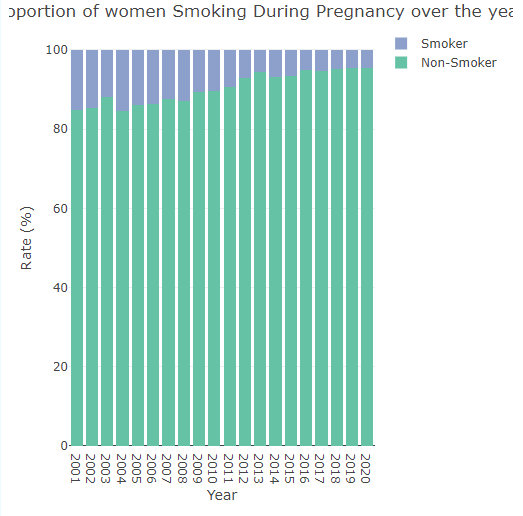
\includegraphics[width=.75\textwidth]{subsections/smoking/smoking_proportion.png}
  \caption{Mother's smoking habit in ACT}
  \label{fig:smoking_prop}
\end{figure}

\subsubsection{Mortality vs Smoking}
As we have discussed previously, smoking is directly related to mortality rate, we came up with an analysis that visualizes how smoking affects different categories of deaths.
We can see in \textbf{Figure \ref{fig:smoking-mortality}} that neonatal death is the highest among mothers who smoked during pregnancy.

\begin{figure}
  \centering
  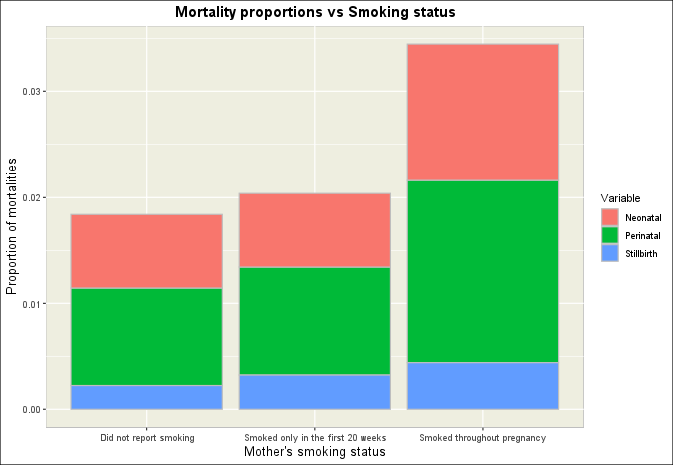
\includegraphics[width=1\textwidth]{subsections/smoking/mortality_vs_smoking.png}
  \caption{neonatal}
  \label{fig:smoking-mortality}
\end{figure}
\subsubsection{Smoker's Age in ACT}
We wanted to find out the correlation between mothers who smoke and their age among the mothers who live in ACT (\textbf{figure \ref{fig:smoking_age}}). We can see that smoking is more common among young mothers. Mothers aged 15-19 are significant in number when it comes to smoking habits. The rate falls drastically as the age increases.
\begin{figure}
  \centering
  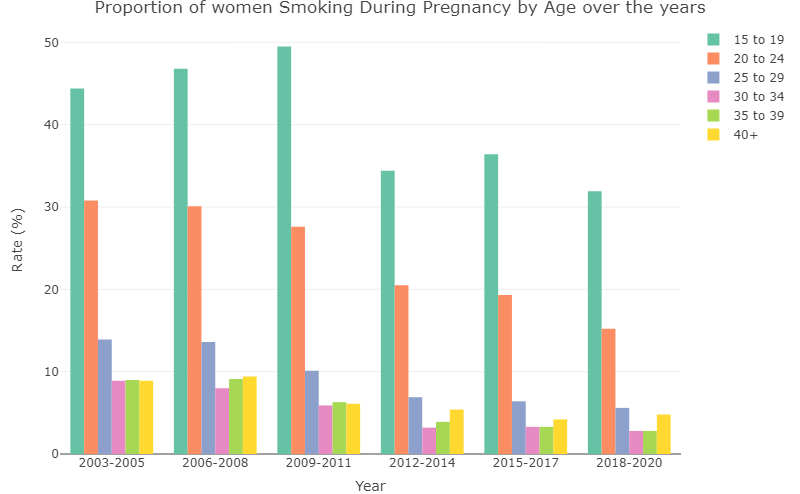
\includegraphics[width=1\textwidth]{subsections/smoking/smoking.png}
  \caption{Age groups of smoking mothers}
  \label{fig:smoking_age}
\end{figure}
\section{Outstanding Issues}
The team had plans to make several machine learning models to predict different matrices of mothers and babies but since the dataset was aggregated and not big enough it was not ideal to make machine learning models based on them. The size of the data was small as well which means that the models would have less accuracy.
\section{Risks Mitigated}
% Risk analysis should include what mitigation IS being taken, by who, and what the resultant (after risk) is. I suggest you use a table with a rating of each risk. These risks are too general for a project report of this nature.
Following are the risks the team predicted and faced during different lifecycles of the project and explained how they were mitigated.

\subsection{Data privacy and security risks} Given the sensitive nature of the data, it was important to ensure that appropriate measures were taken to protect data privacy and security. The data the team used was collected by principally Australian Bureau of Statistics and then aggregated by AIHW. Both of these organizations maintain strict vulnerability and disclosure policies\cite{vulPol} which made sure that the data has abstraction (such as aggregating data) from giving away personal information.

\subsection{Data quality risks} Poor quality data can compromise the accuracy and reliability of the analysis. The datasets that the team had to work on had unorganized data in some of them. Each analysis was done after extracting and compiling the data that was relevant to our objective.

\subsection{Ethical risks} It was important to ensure that the project adheres to ethical principles and guidelines. Since we did not have to collect any data that belonged to an individual or a specific group, the team feels that the analysis is done with proper ethical standards.

\subsection{Project management risks} Effective project management is crucial for ensuring that the project is completed on time and within budget. The team worked on track of previously developed project plans  and followed milestones and timelines. The tasks were delegated among the members appropriately. Also, effective communication and collaboration among team members were ensured.

\subsection{Analysis and interpretation risks} The analysis and interpretation of the data can be influenced by biases, assumptions, and other subjective factors. To mitigate these problems, appropriate statistical methods, conducting sensitivity analyses to assess the impact of different assumptions were performed for each analysis ensuring that the analysis and interpretation are well-documented and transparent.

\section{Lessons Learnt}
Our team came across different challenges and obstacles from the beginning of the project. Our team's learning during this project is twofold.  While in terms of technicality, our learning outcome was not much, in terms of project management our learning was far more significant. The points mentioned below are what the team has learned throughout this journey.
\subsection{Managerial Learning}
\begin{itemize}
    \item It is very important for the team to start the project with a project that is conceptualized properly. The team relocated to this project on week 4 after realizing that the previous project idea was not completely fleshed-out. Since the unit duration is too short the team thought it would be better if we could work on something that is properly conceptualized and the ideas of deliverables are clear to the sponsors. The team communicated with the course coordinators and sponsor and took the necessary steps to work on this project which the team considers a good negotiation skill.
    \item As the principal work with the current sponsor started after week 4 the team had to go through really intense cooperation to catch up with the progress with other groups.
    \item The team had to work on strict deadlines which made other members undertake the responsibilities that were assigned to someone. We consider this as a healthy work ethic.
\end{itemize}
\subsection{Technical Learning}
\begin{itemize}
    \item To work parallelly the team learned to use various collaborative tools like \verb|google colab|, \verb|git|, \verb|github|, etc. 
    \item Gaining access to a workable dataset was extremely limited for this project since it held government data. So the team had to learn the problems and prospects of working with the data that were sensitive.
    \item Our team had to work on a dataset that held aggregated data, which made everything challenging. Each member had to extract and compile the information they were interested in and came up with new datasets from the extracted datasets so that they provided information as robust as the datasets that are not aggregated.
\end{itemize}
\section{Recommendations to the Sponsor}
In our opinion, our sponsor was extremely helpful and communicative. Our sponsor gave us the freedom of choice about what analysis we come up with, what can be the outcome and what are the deliverables. The sponsor also helped the team communicate with the dataset owners from the government agencies which as AIHW. She suggested that should not wait for 2 months for AIHW to give us a fraction of the atomic dataset they own and start working on the aggregated dataset that is publicly accessible. However, the team understands that the analysis would have been more specific if there was access to a more workable dataset that is not aggregated which would allow the team to make better analyses and models for forecasting.
\section{Conclusion}



%% BIBLIOGRAFI %%
\printbibliography[heading=bibintoc]
\newpage

%% VEDLEGG %%

%% DOKUMENT SLUTT %%
\end{document}